\documentclass{beamer}
\usepackage{textpos}
\usepackage{lmodern}
\usepackage{algpseudocode}
\usepackage{amsmath}
\usepackage{tcolorbox}
\usepackage{tikz}
\usepackage{chemarrow}
\usepackage{slashbox}
\usepackage[ruled,linesnumbered]{algorithm2e}
\usepackage{siunitx}
\usepackage{epstopdf}
\usepackage{3dplot}
\usepackage{threeparttable}
\usetikzlibrary{fit}
\usepackage[utf8]{inputenc}
\usepackage[upright]{fourier}
\usetikzlibrary{matrix,arrows,decorations.pathmorphing}
\usepackage{xparse}
\usepackage[nomessages]{fp}% http://ctan.org/pkg/fp
\usetikzlibrary{calc}
\usepackage{breqn} %for dmath
\usepackage{hyperref} 
\usetikzlibrary{shapes,fit}
\definecolor{univred}{rgb}{0.7, 0.0, 0.0}
\DeclareMathOperator*{\argmax}{argmax}
\newcolumntype{C}[1]{>{\centering\let\newline\\\arraybackslash\hspace{0pt}}m{#1}}
\setbeamertemplate{background canvas}{%
    {\color{univred}\noindent\makebox[\paperwidth]{\rule{\paperwidth}{2.5ex}}
}}
\setbeamertemplate{frametitle}{\color{black}\bfseries\vskip2ex\insertframetitle\par\vskip-6pt\hrulefill}
%\usepackage{pgfpages}
%\setbeameroption{show notes}
%\setbeameroption{show notes on second screen=right}
\addtobeamertemplate{frametitle}{}{%
%CMU logo in header
    \begin{textblock*}{100mm}(0.87\textwidth,-1.425cm)
        \includegraphics[height=1.5cm,width=1.9cm,keepaspectratio]{cm_logo}
    \end{textblock*}
%ECE logo in footer
    \begin{textblock*}{10mm}(-.8cm,7.5cm)
        \includegraphics[height=2cm,width=2.5cm,keepaspectratio]{ece}
    \end{textblock*}
}
\addtobeamertemplate{footnote}{}{\vspace{2ex}}
\setbeamercolor*{item}{fg=black}
\setbeamertemplate{footline}[page number]{}
\setbeamercolor{page number in head/foot}{fg=univred}
%for matrix mul.
\newcommand{\myunit}{0.6 cm}
\tikzset{
    node style sp/.style={draw,circle,minimum size=\myunit},
    node style ge/.style={circle,minimum size=\myunit},
    arrow style mul/.style={draw,sloped,midway,fill=white},
    arrow style plus/.style={midway,sloped,fill=white},
}
%end
% for rowvectors and column vectors
\ExplSyntaxOn
\NewDocumentCommand{\Rowvec}{ O{,} m }
{
    \vector_main:nnnn { p } { & } { #1 } { #2 }
}
\NewDocumentCommand{\Colvec}{ O{,} m }
{
    \vector_main:nnnn { p } { \\ } { #1 } { #2 }
}
%end
\seq_new:N \l__vector_arg_seq
\cs_new_protected:Npn \vector_main:nnnn #1 #2 #3 #4
{
    \seq_set_split:Nnn \l__vector_arg_seq { #3 } { #4 }
    \begin{#1matrix}
        \seq_use:Nnnn \l__vector_arg_seq { #2 } { #2 } { #2 }
    \end{#1matrix}
}
\ExplSyntaxOff
\newcommand{\highlight}[1]{%
    \colorbox{red!50}{$\displaystyle#1$}}
    \title{\color{univred} A Comparison of Antenna Placement Algorithms}
    \author{Abhinav Jauhri}
    \date{\today}
    \begin{document}
    \begin{frame}
        \color{univred}
        \titlepage
    \end{frame}

    \begin{frame}[t]{Motivation}
        \begin{itemize}
            \item<1->Multiple antenna placement on a platform is a manual, and time consuming process
            \item<2->Number of possible placements (search space) of antennas becomes exponentially large in the number of antennas to be placed
            \item<3-> Stochastic algorithms have been used effectively to find antenna designs {\textit{\small (Reference: Hornby, Lohn, \& Linden. "Computer-Automated Evolution of an X-Band Antenna for NASA's Space Technology 5 Mission." 2011)}}
        \end{itemize}
        \vspace{5mm}
        \centering\only<4->{How can we automate the process by use of stochastic algorithms?}
    \end{frame}
 
    \begin{frame}[t]{Contributions}
        \begin{itemize}
            \item Formulation of the antenna placement problem
            \item Evaluation of standard stochastic algorithms on a real-world problem
            \item Able to achieve global optimum with as low as 21\% evaluations
        \end{itemize}
        \vspace{5mm}
    \end{frame}
   

    \begin{frame}[t]{Antenna Placement Example}
        \begin{figure}
            \centering
            \includegraphics[width=.6\textwidth]{car.png}
        \end{figure}
        \begin{itemize}
            \item \textcolor{red}{$A_1$} has $24$ possible antenna placements
            \item \textcolor{cyan}{$A_2$} has $33$ possible antenna placements
            \item \textcolor{black}{$A_3$} has $136$ possible antenna placements
        \end{itemize}
        Size of search space $= m^n$, where $m$ is the number of allowable placements for one antenna, and $n$ is the number of antennas.
    \end{frame}

    \begin{frame}[t]{Antenna Placement Problem}
        Given:
    \begin{itemize} \itemsep1.5em
            \item<1-> platform $P$ with its surface gridded such that end points represent possible antenna placement
            \item<2-> set of  $m~(m > 1)$ antennas $A = {A_1, A_2, \dots, A_m}$
            \item<3-> for each $A_i$, let $L_i$ denote the set of allowable placements locations $\in \mathbb R^3$ such that $\mid L_i \mid = n_i$ and $\forall i, n_i > 1$; $L_i = \{(x_{1}, y_{1}, z_{1}) \dots (x_{n_i}, y_{n_i}, z_{n_i})\}$
        \end{itemize}
        \vspace{10px}
        \centering\only<4->{\textbf{Goal}: Find a set of $n$ antenna locations on $P$}
    \end{frame}

    \begin{frame}[t]{Stochastic Algorithms}
        We will consider algorithms which rely on \textit{randomization} principle.
        \vspace{10px}
    \begin{itemize} \itemsep1.5em
            \item Simple Genetic Algorithm
            \item Evolutionary Strategy
            \item Simulated Annealing
            \item Hill Climbing
        \end{itemize}
    \end{frame}

    \begin{frame}[t]{Characterstics of Stochastic Algorithms}
    \begin{itemize} \itemsep1.5em
            \item A set of solution candidates (or hypothesis) maintained
            \item Mating selection process is performed on the solution candidates
            \item Several solutions are combined to generate new candidate solutions
        \end{itemize}
    \end{frame}



    \begin{frame}[t]{Representation}
        \begin{figure}
            \centering
            \includegraphics[width=.6\textwidth]{car.png}
        \end{figure}
        A hypothesis is represented by a set of antenna placements. For instance - $(\textcolor{red}{(x_i, y_i, z_i)}, \textcolor{cyan}{(x_j, y_j, z_j)}, \textcolor{black}{(x_k, y_k, z_k)})$
    \end{frame}

    \begin{frame}[t]{Evolutionary Strategy}
        \fontsize{8}{12}\selectfont
        \begin{algorithm}[H]
%\scriptsize
            \KwData{Set of placements $L=\{L_1, \cdots, L_m\}$; $\mu$; $\lambda$; $gen_{max}$ - maximum number of generations}
            \KwResult{$H^*$ from $P$ }
            Initialize $P\leftarrow$ generate $\mu$ random hypothesis \;
            $gen_{id}=0$ \;
            \While{$gen_{id}<gen_{max}$} {
                Create $\lambda / \mu$ offsprings from  each $\mu$ hypotheses by applying mutation operator, and add all offsprings to $P$ \;
                Compute the $fitness(h_i), i=1,\ldots, \lambda$ \;
                Keep $\mu$ best hypotheses in P, and discard remaining $\lambda - \mu$ hypotheses \;
                Update $gen_{id} \leftarrow gen_{id}+1$
            }
            \caption{AP-ES}
        \end{algorithm}
    \end{frame}

    \begin{frame}[t]{Simulated Annealing}
        \fontsize{8}{8}\selectfont
        \begin{algorithm}[H]
%\scriptsize
            \KwData{Set of placements $L=\{L_1, \cdots, L_m\}$; $T$ - initial temperature; $i_{m}$ - maximum iterations; $f_{cooling}$ - cooling factor }
            \KwResult{$H^*$ from $P$}
            Initialize $H\leftarrow$ generate a random hypothesis \;
            Compute $fitness(H)$  \;
            $i=0$ \;
            \While{$i<i_m$} {
                Mutation - Apply the operation on $H$ as stated in Algorithm . Call the pertubrated/mutated hypothesis $C$ \;
                Compute $\delta f = fitness(C) -fitness(H) $ \;
                \eIf{$\delta f > 0$} {
                    Generate a random number $\epsilon$ using a uniform distribution over $[0,1]$ \;
                    \If{$\epsilon < e^{-\delta f / T}$} {
                        $H \leftarrow C$
                    }}  {
                    $H \leftarrow C$ \; }
                    $T \leftarrow T \cdot f_{cooling}$ \;
                    $i \leftarrow i + 1$ \;
                } 
                \caption{AP-SA}
                \label{alg:ap-sa}
            \end{algorithm}
        \end{frame}

        \begin{frame}{Minimize Difference in Radiation Pattern}
            Pattern defines the ratio of energy radiated and input energy in a particular direction. For each antenna $A_i$:
            \begin{tcolorbox}[colback=green!5]
                \begin{equation} \label{eq:rp}
                    F_{RP}(A_i) = \sum_{\theta}\sum_{\phi} 
                    \| FSG_i(\theta,\phi) - ISG_i(\theta,\phi) \| ^2,
                \end{equation}
            \end{tcolorbox}
            where
            \begin{itemize}
                    \small
                \item $\theta, \phi$ spherical and cylindrical coordinates
                \item $FSG(\cdot)$ returns free-space gain pattern  
                \item $ISG(\cdot)$ returns in-situ gain pattern
            \end{itemize}

            \tdplotsetmaincoords{60}{110}
            \pgfmathsetmacro{\rvec}{.8}
            \pgfmathsetmacro{\thetavec}{30}
            \pgfmathsetmacro{\phivec}{60}
            \hspace{.6\textwidth}
                \begin{tikzpicture}[scale=1.8,tdplot_main_coords]
    \tikzstyle{every node}=[font=\tiny]
                    \coordinate (O) at (0,0,0);
                    \tdplotsetcoord{P}{\rvec}{\thetavec}{\phivec}
                    \draw[thick,->] (0,0,0) -- (1,0,0) node[anchor=north east]{$x$};
                    \draw[thick,->] (0,0,0) -- (0,1,0) node[anchor=north west]{$y$};
                    \draw[thick,->] (0,0,0) -- (0,0,1) node[anchor=south]{$z$};
                    \draw[-stealth,color=red] (O) -- (P);
                    \draw[dashed, color=red] (O) -- (Pxy);
                    \draw[dashed, color=red] (P) -- (Pxy);
                    \tdplotdrawarc{(O)}{0.2}{0}{\phivec}{anchor=north}{$\phi$}
                    \tdplotsetthetaplanecoords{\phivec}
                    \tdplotdrawarc[tdplot_rotated_coords]{(0,0,0)}{0.5}{0}{\thetavec}{anchor=south west}{$\theta$}
                    \draw[dashed,tdplot_rotated_coords] (\rvec,0,0) arc (0:90:\rvec);
                    \draw[dashed] (\rvec,0,0) arc (0:90:\rvec);
                \end{tikzpicture}
        \end{frame}


        \begin{frame}{Minimize Coupling}
            Coupling is the absorption of radiated energy by nearby antennas
            \begin{tcolorbox}[colback=green!5]
                \begin{equation}
                    F_{MC} = \sum_{i=1}^{m-1}\sum_{j=i+1}^{m} CP(A_i, A_j),
                \end{equation}
            \end{tcolorbox}
            where
            \begin{itemize}
                \item $CP(\cdot)$ computes the coupling between two antennas
                \item $i \neq j$
            \end{itemize}
        \end{frame}


        \begin{frame}{Overall Fitness Function}
            For an hypothesis, fitness is defined as:
            \begin{tcolorbox}[colback=green!5]
                \begin{equation} \label{eq:optimal}
                    F = \alpha F_{MC} + \beta \sum_{i} F_{RP}(A_i),
                \end{equation}
            \end{tcolorbox}
            where $\alpha + \beta = 1$
        \end{frame}


        \begin{frame}[t]{Experimental Setup}
            \begin{enumerate}
                \item Create (s) such that each individual is defined by a placement for each of the $m$ antennas
                \item Run all individuals through \textit{NEC} simulator \footnote{http://www.nec2.org} to get fitness parameters 
                \item Apply EA operators 
                \item Repeat till either global minimum is reached or 50\% evaluations of search space
            \end{enumerate}
            \vspace{10mm}
        \end{frame}

        \begin{frame}{Experiments: Test Cases}
            \begin{table}
                \centering
                \begin{tabular}{|c|c|c|} \hline
                    Test Case&Antennas&Total allowable placements\\ \hline
                    1 & 2 & 7,056 (83x83) \\ \hline
                    2 & 3 & 50,625 (45x45x25) \\ \hline
                    3 & 3 & 126,025 (71x71x25) \\ \hline
                    4 & 4 & 20,736 (12x12x12x12) \\
                    \hline\end{tabular}
            \end{table}
            \small *Allowable placements for each antenna are provided within parenthesis
        \end{frame}

        \begin{frame}{Results - Success Probability}
            \begin{center}
                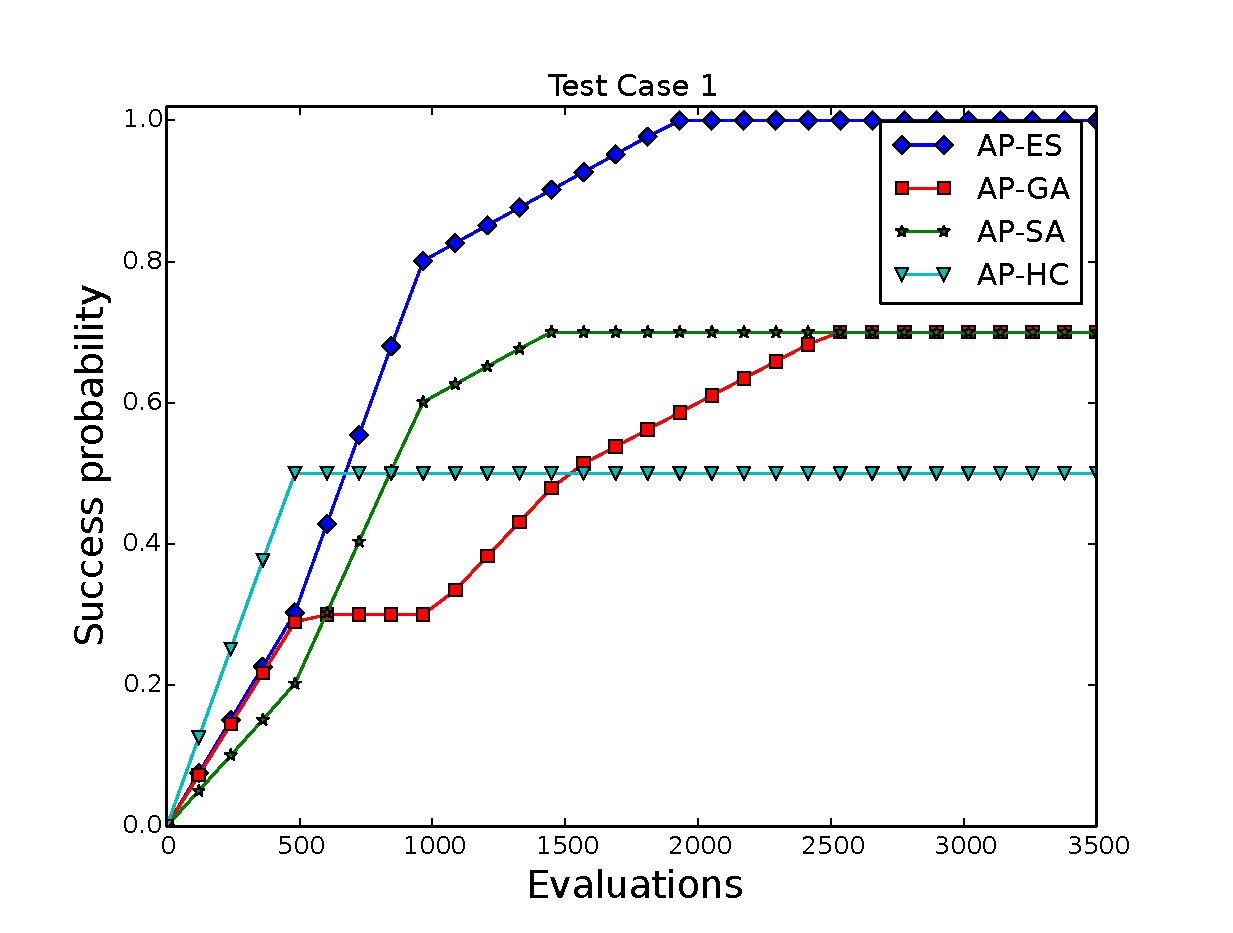
\includegraphics[width=.49\textwidth]{../paper/FIG/tc1_sp.eps}
                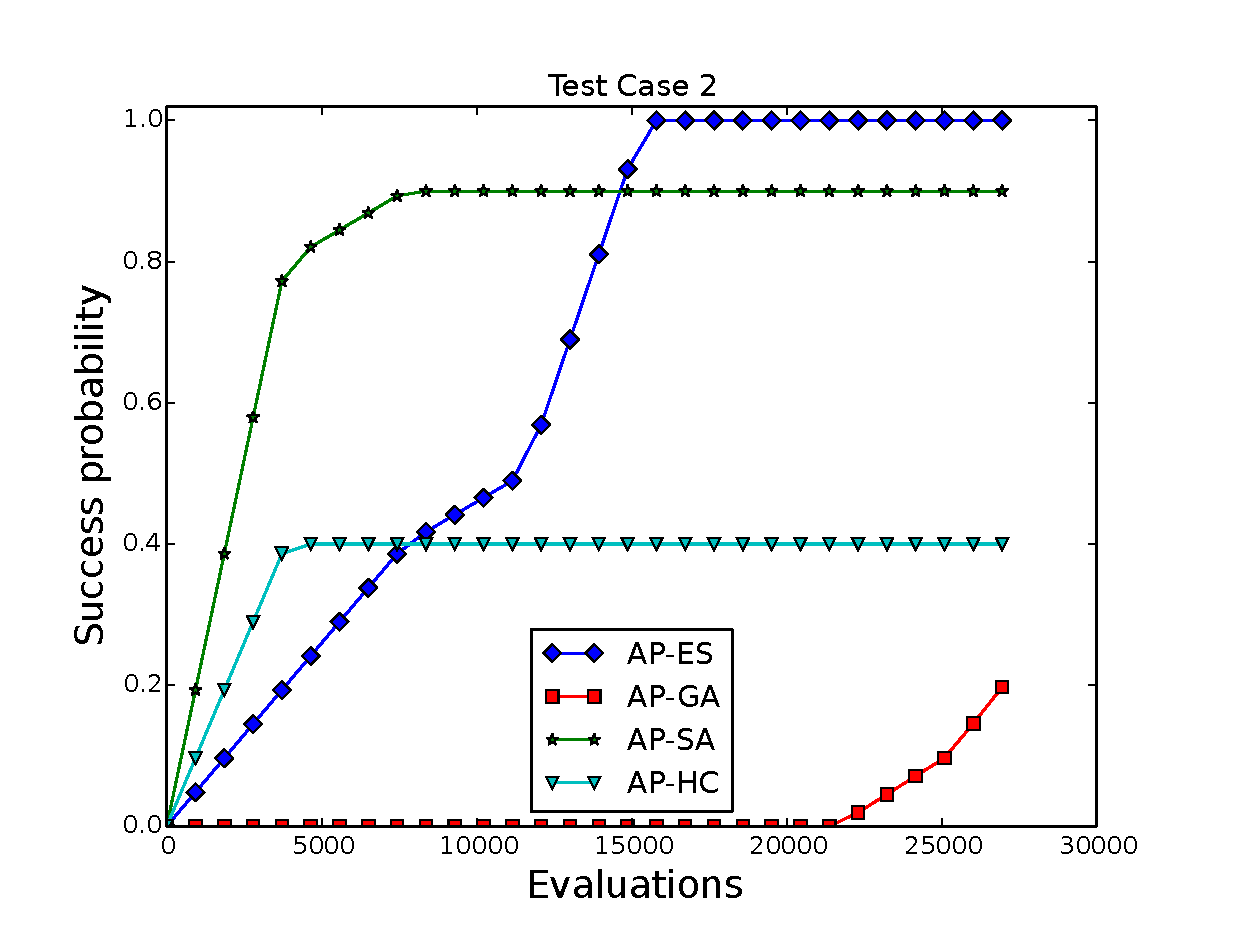
\includegraphics[width=.49\textwidth]{../paper/FIG/tc2_sp.eps}
            \end{center}
        \end{frame}

        \begin{frame}{Results - Success Probability}
            \begin{center}
                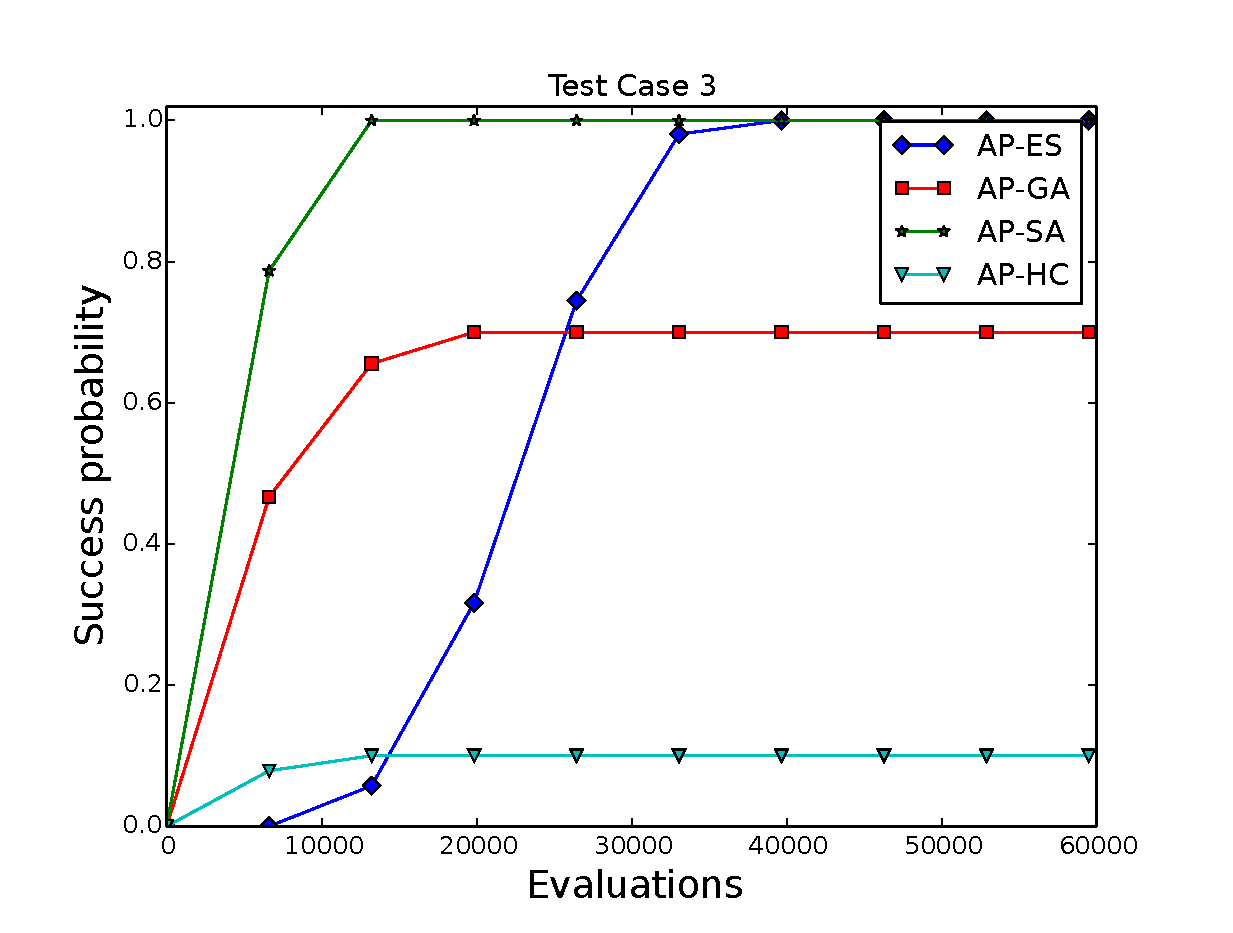
\includegraphics[width=.49\textwidth]{../paper/FIG/tc3_sp.eps}
                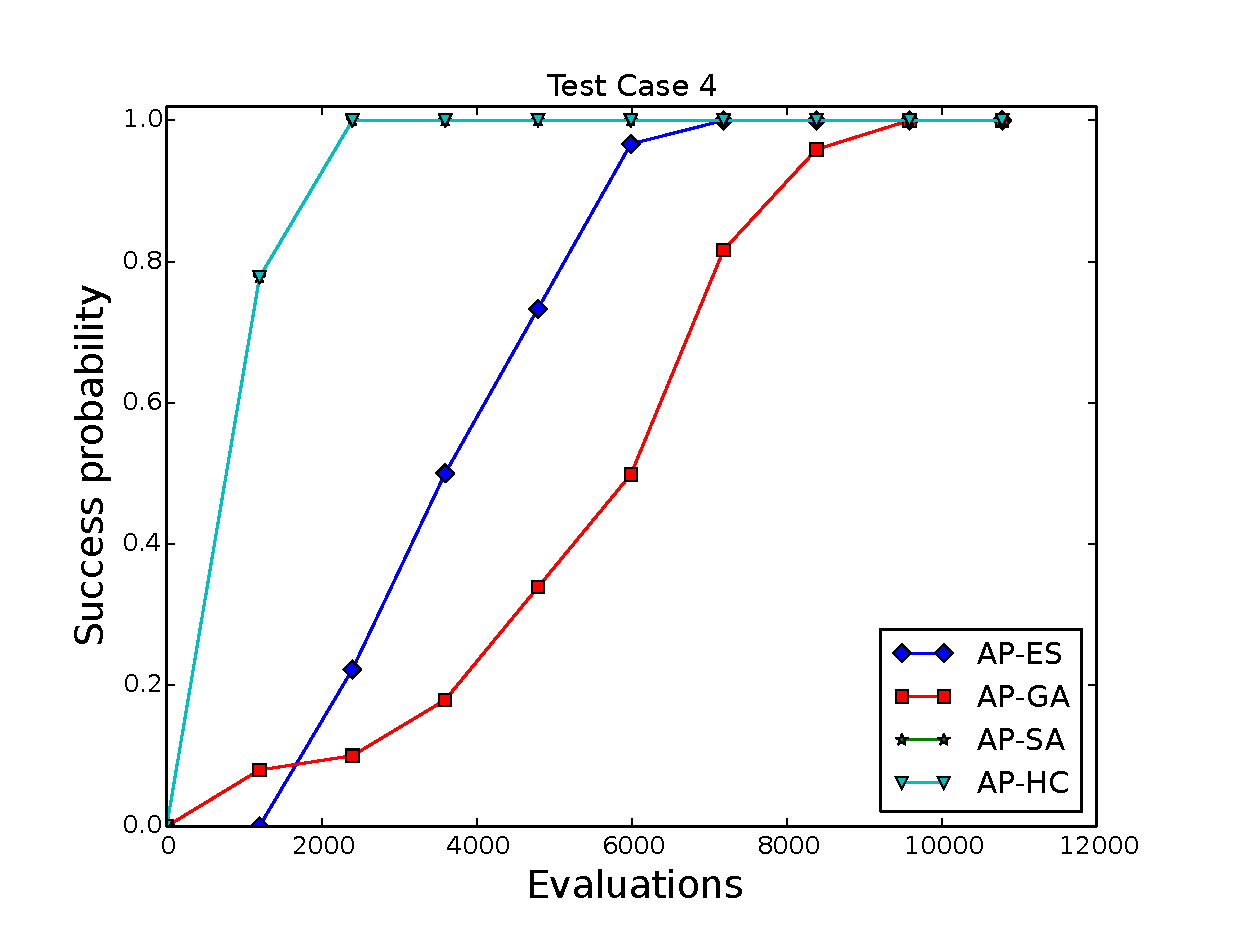
\includegraphics[width=.49\textwidth]{../paper/FIG/tc4_sp.eps}
            \end{center}
        \end{frame}

        \begin{frame}{Equivalence of fitness to efficiency}
            \small For a particular test case, fitness change of $0.01$ is equivalent to either the corresponding value under expected gain ($\mathbb E_g$) column, or difference in coupling ($\Delta_c$).
            \begin{table}
                \centering
                \begin{threeparttable}
                    \begin{tabular}{|C{1cm}|C{2.5cm}|C{2.5cm}|} \hline
                        ID& $\mathbb E_g$ & $\Delta_{c}$ (dB) \\ \hline
                        tc1 & 872.277 & 0.5474 \\ \hline
                        tc2 & 862.082 & 1.3034 \\ \hline
                        tc3 & 861.845 & 1.5180 \\ \hline
                        tc4 & 871.049 & 0.5693 \\
                        \hline\end{tabular}
                \end{threeparttable}
            \end{table}
            \tiny
            $\mathbb E_g = \frac{1}{N \cdot m} \sum_{i}^m F_{RP}(A_i),$
            where $N = \;\mid \theta \mid \cdot \mid \phi \mid$
        \end{frame}

        \begin{frame}{Conclusion}
            \begin{itemize}
                \item Formulation of the antenna placement problem
                \item Generic problem formulation to accommodate multiple antennas and platforms
                \item Optimal placements found using stochastic algorithms
            \end{itemize}
        \end{frame}

        \end{document}
